\chapter{Introduction}
%\thispagestyle{plain} 

\section{Key Terms}
\subsection{The Components of Storm}
In a Storm cluster, nodes are organized into a master node that runs continuously. There are two kind of nodes in a Storm cluster: master node and worker nodes. Master node run a daemon called Nimbus, which is responsible for distributing code around the cluster, assigning tasks to each worker node, and monitoring for failures. Worker nodes run a daemon called Supervisor, which executes a portion of a topology. A topology in Storm runs across many worker nodes on different machines. Since Storm keeps all cluster states either in Zookeeper or on local disk, the daemons are stateless and can fail or restart without affecting the health of the system.
\begin{center}
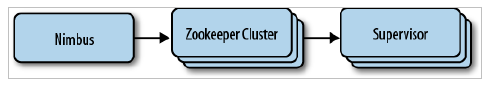
\includegraphics[scale=.5]{../img/img1}\\[2mm]
\end{center}
{\bfseries Properties of Storm}\\[2mm]
Within all these design concepts and decisions, there are some really nice properties that make Storm unique.\\[2mm]
{\bfseries Simple to program}\\[2mm]
Doing real-time processing from scratch is very painful. With Storm, complexity is dramatically reduced.\\[2mm]
{\bfseries Support for multiple programming languages}\\[2mm]
It's easier to develop in a JVM-based language, but Storm supports any language as long as a a small intermediary library is used or implemented.\\[2mm]
{\bfseries Fault-tolerant}\\[2mm]
The Storm cluster takes care of workers going down, reassigning tasks when necessary.\\[2mm]
{\bfseries Scalable}\\[2mm]
All one need to do in order to scale is add more machines to the cluster. Storm will
reassign tasks to new machines as they become available.\\[2mm]
{\bfseries Reliable}\\[2mm]
All messages are guaranteed to be processed at least once. If there are errors, messages
might be processed more than once, but messages will never be lost.\\[2mm]
{\bfseries Fast}\\[2mm]
Speed was one of the key factors driving Storm's design.\\[2mm]
{\bfseries Transactional}\\[2mm]
One can get exactly once messaging semantics for pretty much any computation.\\[2mm]

\subsection{Operational Modes}
There are two ways to run Storm.\\[2mm]
{\bfseries Local Mode}\\[2mm]
n Local Mode, Storm topologies run on the local machine in a single JVM. This mode is used for development, testing, and debugging because it's the easiest way to see all topology components working together. In this mode, we can adjust parameters that enable us to see how our topology runs in different Storm configuration environments.To run topologies in Local Mode, we'll need to download the Storm development dependencies, which are all the things that we need to develop and test our topologies.Running a topology in Local Mode is similar to running it in a Storm cluster. However it's important to make sure that all components are thread safe, because when they are deployed in Remote Mode they may run in different JVMs or on different physical machines without direct communication or shared memory.\\[2mm]
{\bfseries Remote Mode}\\[2mm]
In Remote Mode, we submit our topology to the Storm cluster, which is composed of many processes, usually running on different machines. Remote Mode doesn't show debugging information, which is why it's considered Production Mode. However, it is possible to create a Storm cluster on a single development machine, and it's a good idea to do so before deploying to production, to make sure there won't be any problems running the topology in a production environment.\\[2mm]
\subsection{Storm Topology}
\begin{center}
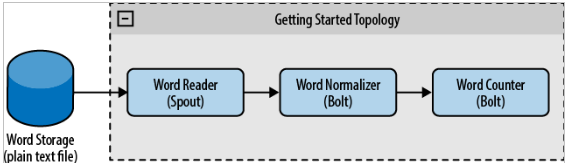
\includegraphics[scale=.5]{../img/img2} \\[2mm]
\end{center}
The logic for a real-time application is packaged into a Storm topology. A Storm topology is analogous to a MapReduce job. One key difference is that a MapReduce job eventually finishes, whereas a topology runs forever (or until you kill it, of course). A topology is a graph of spouts and bolts that are connected with stream groupings.
\subsection{Understanding of Basic Terms}
{\bfseries Streams}\\[2mm]
The stream is the core abstraction in Storm. A stream is an unbounded sequence of tuples that is processed and created in parallel in a distributed fashion. Streams are defined with a schema that names the fields in the stream's tuples. By default, tuples can contain integers, longs, shorts, bytes, strings, doubles, floats, booleans, and byte arrays. You can also define your own serializers so that custom types can be used natively within tuples.\\[2mm]
{\bfseries Spout}
A spout is a source of streams in a topology. Generally spouts will read tuples from an external source and emit them into the topology (e.g. a Kestrel queue or the Twitter API). Spouts can either be reliable or unreliable. A reliable spout is capable of replaying a tuple if it failed to be processed by Storm, whereas an unreliable spout forgets about the tuple as soon as it is emitted.\\[1mm]
Spouts can emit more than one stream. To do so, declare multiple streams using the declareStream method of OutputFieldsDeclarer and specify the stream to emit to when using the emit method on SpoutOutputCollector.\\[1mm]
The main method on spouts is nextTuple. nextTuple either emits a new tuple into the topology or simply returns if there are no new tuples to emit. It is imperative that nextTuple does not block for any spout implementation, because Storm calls all the spout methods on the same thread.The other main methods on spouts are ack and fail. These are called when Storm detects that a tuple emitted from the spout either successfully completed through the topology or failed to be completed.ack and fail are only called for reliable spouts.\\[2mm]
{\bfseries Direct Connection}\\[2mm]
In a direct connection architecture, the spout connects directly to a message emitter.
\begin{center}
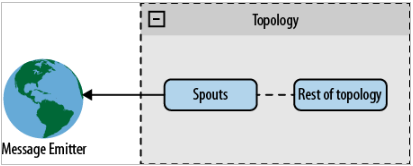
\includegraphics[scale=.5]{../img/img3} \\[2mm]
\end{center}
This architecture is simple to implement, particularly when the message emitter is a well-known device or a well-known device group. A well-known device is one that is known at startup and remains the same throughout the life of the topology.\\[2mm]
{\bfseries Bolts}\\[2mm]
All processing in topologies is done in bolts. Bolts can do anything from filtering, functions, aggregations, joins, talking to databases, and more.
Bolts can do simple stream transformations. Doing complex stream transformations often requires multiple steps and thus multiple bolts. For example, transforming a stream of tweets into a stream of trending images requires at least two steps: a bolt to do a rolling count of retweets for each image, and one or more bolts to stream out the top X images.\\[2mm]
{\bfseries Bolt Lifecycle}\\[2mm]
A bolt is a component that takes tuples as input and produces tuples as output. Bolts are created on the client machine, serialized into the topology, and submitted to the master machine of the cluster. The cluster launches workers that deserialize the bolt, call prepare on it, and then start processing tuples. To customize a bolt, one should set parameters in its constructor and save them as instance variables so they will be serialized when submitting the bolt to the cluster. When writing a bolt, usually IRichBolt interface is implemented.\\[2mm]
{\bfseries Bolt Structure}\\[2mm]
Bolts have the following methods:\\[2mm]
declareOutputFields(OutputFieldsDeclarer declarer)\\[2mm]
Declare the output schema for this bolt\\[2mm]
prepare(java.util.Map stormConf, TopologyContext context, OutputCollector collector)\\[2mm]
Called just before the bolt starts processing tuples\\[2mm]
execute(Tuple input)\\[2mm]
Process a single tuple of input\\[2mm]
cleanup()\\[2mm]
Called when a bolt is going to shut down.

\subsection{Different Grouping}
{\bfseries Streams Groupings}\\[2mm]
Part of defining a topology is specifying for each bolt which streams it should receive as input. A stream grouping defines how that stream should be partitioned among the bolt's tasks.There are seven built-in stream groupings in Storm, and one can implement a custom stream grouping by implementing the  CustomStreamGrouping  interface:\\[2mm]
{\bfseries Shuffle grouping:} Tuples are randomly distributed across the bolt's tasks in a way such that each bolt is guaranteed to get an equal number of tuples.\\[2mm]
{\bfseries Fields grouping:} The stream is partitioned by the fields specified in the grouping. For example, if the stream is grouped by the "user-id" field, tuples with the same "user-id" will always go to the same task, but tuples with different "user-id"'s may go to different tasks.\\[2mm]
{\bfseries All grouping:} The stream is replicated across all the bolt's tasks. This grouping should be with care.\\[2mm]
{\bfseries Global grouping:} The entire stream goes to a single one of the bolt's tasks. Specifically, it goes to the task with the lowest id.\\[2mm]
{\bfseries None grouping:} This grouping specifies that you don't care how the stream is grouped. Currently, none groupings are equivalent to shuffle groupings. Eventually though,Storm will push down bolts with none groupings to execute in the same thread as the bolt or spout they subscribe from (when possible).\\[2mm]
{\bfseries Direct grouping:} This is a special kind of grouping. A stream grouped this way means that the producer of the tuple decides which task of the consumer will receive this tuple. Direct groupings can only be declared on streams that have been declared as direct streams. Tuples emitted to a direct stream must be emitted using one of the emitDirect methods. A bolt can get the task ids of its consumers by either using the provided TopologyContext or by keeping track of the output of the emit method in OutputCollector(which returns the task ids that the tuple was sent to).\\[2mm]
{\bfseries Local or shuffle grouping:} If the target bolt has one or more tasks in the same worker process, tuples will be shuffled to just those in-process tasks. Otherwise, this acts like a normal shuffle grouping.\\[2mm]

\section{Aim and Objective} 
\subsection{Aim}
To implement stateful bolts in storm.
\subsection{Objective}
Storm is one of the most watched projects on github and its popularity lies in the fact that real-time processing is a need of the hour. It is important for real-time processing to reduce redundant computation in order to increase the throughput and response time. Our objective is to make stateful bolts in Storm which are at the moment stateless so that redundant computation is reduced thus improving the throughput and response time.

